\section{Wires}

On a schematic a wire is a perfect conductor. Electricity flows without loss or degredation. (To be fair, scientists are working on superconductor technology that mimics this behavior. Currently, such systems are limited to conditions that include cooling the materials to incredibly cold temperatures.)

The most basic parasitic effect of wires is resistance. Copper, the most common wiring material, has a resistivity of $1.68 \dot 10^{-8} \Omega m$. The next most common wiring element, aluminum, is over 50\% more resistive, but is lighter and cheaper. Silver is actually the most conductive element, beating copper by about 5\%, but is expensive and tarnishes easily. Gold is on par with aluminum for resistance, but has excellent anti-corrosion properties and thus is heavily used in connectors that get exposed to air.

When the term ``wire'' is used here, you may often think of a simple cylinder of copper in a plastic sheath that is found in the walls. In truth, all these principles apply to any metal that is used to carry current from one point to another, including PCB traces, component leads, circuit chip bond wires, and more.

The resistance values mentioned above are with regards to DC current. AC current is another matter: as the frequency of the current through a conductor increases, the current tends to cluster at its outside edges. This reduces the effective amount of metal that the current is flowing through, and increases the effective resistance. Figure \ref{skin_depth}\footnote{Image is in public domain. Created by Wikipedia user ``Biezl'' on 2008-July-27.} shows how high-frequency current mostly flows through the outer portion of a conductor (darker red shading is more current density).


\begin{figure}[h]
\centering
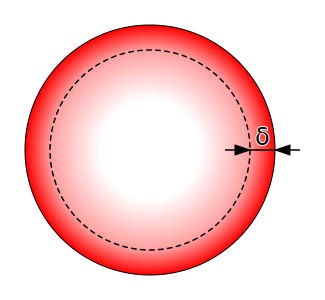
\includegraphics[scale=0.5]{skin_depth.png}
\caption{Skin Depth for HF Current}\label{skin_depth}
\end{figure}

The reason for this is how electrical current creates magnetic fields, and then magnetic fields oppose the flow of current. At its most basic level, current through a wire creates a magnetic field perpendicular to and surrounding the wire. See Figure \ref{wire_mag_field} for a simplified diagram of this effect; electrical current is in blue and magnetic flux is in red.

\begin{figure}[h]
\centering
\includegraphics[scale=0.5]{wire_mag_field.png}
\caption{Wire Current and Magnetic Field}\label{wire_mag_field}
\end{figure}

This same effect happens throughout the cross-section of a wire carrying AC current. AC current through one portion of the wire creates a magnetic field that affects the current in surrounding portions. The magnetic field increases the effective resistance of the wire (really, complex reactance). Magnetic fields on the outer edge of the conductor (see Figure \ref{skin_fields}\footnote{Image is in public domain. Created by Wikipedia user ``Biezl'' on 2008-July-27.}) permeate into the air and thus have less strength than those in the middle.

\begin{figure}[h]
\centering
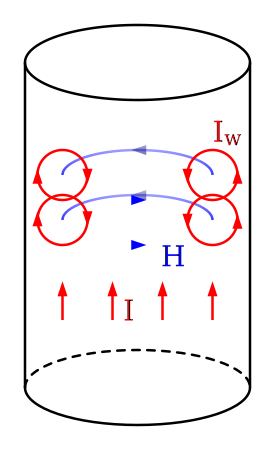
\includegraphics[scale=0.5]{skin_effect_fields.png}
\caption{Magnetic Fields In Wire}\label{skin_fields}
\end{figure}